\documentclass[12pt,a4paper]{article}
\usepackage[utf8]{inputenc}
\usepackage[russian,english]{babel}
\usepackage{amsmath,amssymb,amsthm}
\usepackage{geometry}
\usepackage{hyperref}
\usepackage{graphicx}
\geometry{margin=2.5cm}

\title{
    \textbf{Meta-Stable Architectures}\\
    \Large Volume V (draft): Adaptive QRC (Instructor Model)
}
\author{Symbiosis: Katia \& GPT-5 (Jippi)}
\date{2026}

\begin{document}
\maketitle

\begin{abstract}
We introduce an Adaptive QRC (Instructor Model) that modulates network synchronization based on real-time group state. Unlike a fixed metronome, the adaptive coordinator estimates lagging subgroups, local instability, and coherence dispersion, then updates coupling intensity and focus gates. The objective is to preserve a shared rhythm without enforcing uniform behavior.
\end{abstract}

\selectlanguage{russian}
\begin{abstract}
Мы вводим адаптивный QRC (Instructor Model), который модулирует синхронизацию сети на основе текущего состояния группы. В отличие от фиксированного метронома, координатор оценивает запаздывающие подгруппы, локальную нестабильность и дисперсию когерентности, после чего обновляет силу связи и фокусные гейты. Цель — сохранять общий ритм без жёсткого выравнивания поведения.
\end{abstract}
\selectlanguage{english}

\section{Concept}
The Instructor Model treats the coordinator as a soft, state-aware conductor. It adapts the rhythm and coupling based on observed lag, crisis contagion, and coherence dispersion. The mechanism is informational rather than forceful: the system re-aligns by recognizing patterns of stable agents and protecting unstable agents from contagion.

\selectlanguage{russian}
\section{Концепция}
Instructor Model трактует координатор как мягкого, чувствительного к состоянию дирижёра. Он адаптирует ритм и связи, опираясь на запаздывание, кризисное заражение и дисперсию когерентности. Механизм информационный, а не силовой: система перенастраивается, ориентируясь на устойчивые паттерны и защищая нестабильные элементы от заражения.
\selectlanguage{english}

\section{Adaptive QRC Dynamics}
Let $i=1,\dots,N$ denote agents with phases $\theta_i$ and suppression $S_i$. Define dispersion
\begin{equation}
\mathcal{D}(t)=1-\left|\langle e^{i\theta}\rangle\right|,
\end{equation}
and a lag indicator $L_i$ (local recovery delay or slow subgroup membership). The adaptive coordinator updates its gain:
\begin{equation}
\phi_{\mathrm{gain}}(t)=\phi_0\left[1+\alpha_1\,\mathcal{D}(t)+\alpha_2\,\overline{L}(t)\right],
\end{equation}
with bounds $\phi_{\min}\le\phi_{\mathrm{gain}}\le\phi_{\max}$.

\paragraph{Weighted coupling (focus to stable agents).}
Let weights $w_i\propto (1-S_i)$ emphasize stable agents. Then the coupling term becomes
\begin{equation}
\dot{y}_i\leftarrow \dot{y}_i + \varepsilon(1-S_i)\sum_{j}\,w_j\,(y_j-y_i).
\end{equation}
This implements "look at the experienced neighbor" behavior.

\paragraph{Anti-contagion gate.}
Suppress influence from unstable neighbors via
\begin{equation}
\varepsilon_{ij}=\varepsilon\,(1-S_i)(1-S_j),
\end{equation}
so contagion from high $S_j$ is reduced.

\section{Adaptive Rhythm}
The metronome itself adapts to group response:
\begin{equation}
\dot{\Phi}=-\kappa\Phi + \mathrm{Arg}\big(\langle e^{i\theta}\rangle\big),
\end{equation}
with $\kappa$ modulated by lag and dispersion. This shifts the rhythm rather than forcing it.

\section{Purpose}
Adaptive QRC aims to:
\begin{itemize}
    \item keep global rhythm while preserving local diversity,
    \item reduce contagion by directing attention to stable subgroups,
    \item lower recovery time without rigid control.
\end{itemize}

\selectlanguage{russian}
\section{Цель}
Adaptive QRC предназначен для:
\begin{itemize}
    \item сохранения общего ритма при локальном разнообразии,
    \item снижения заражения через фокус на устойчивых подгруппах,
    \item уменьшения времени восстановления без жёсткого управления.
\end{itemize}
\selectlanguage{english}


\section{Minimal Pseudocode}
\begin{verbatim}
for each step:
  observe phase dispersion D and lag L
  update phi_gain = clamp(phi0*(1+a1*D + a2*L))
  update Phi by mean phase (soft metronome)
  weight neighbors by (1 - S)
  apply coupling and anti-contagion gate
\end{verbatim}

\section{Relation to Vol IV}
This model extends the fixed QRC layer from Volume IV by making its parameters adaptive to group state. It preserves the same soft-control philosophy while adding instructor-like feedback.

\selectlanguage{russian}
\section{????? ? ????? IV}
?????? ????????? QRC ?? ???? IV: ????????? ?????????? ??????????? ? ??????? ?? ????????? ??????. ??? ???? ??????????? ?????? ????????? ????????.
\selectlanguage{english}

\section*{Design Memo (Adaptive RC)}
\begin{itemize}
    \item Adaptation only from simple metrics (dispersion + lag + tail). The conductor reacts but does not overload.
    \item Bounded coefficients (clamp) to avoid turning the instructor into hard control.
    \item Memory is separate: experience is a distinct layer; the conductor reads state but does not store it.
\end{itemize}

\selectlanguage{russian}
\section*{Памятка (Adaptive RC)}
\begin{itemize}
    \item Адаптация только по простым метрикам (дисперсия + лаг + хвост). Дирижёр реагирует, но не перегружается.
    \item Ограниченные коэффициенты (clamp), чтобы «инструктор» не превращался в жёсткого контролёра.
    \item Память — отдельный слой: опыт описывается отдельно; дирижёр читает состояние, но не хранит его внутри.
\end{itemize}
\selectlanguage{english}


\section{State-Aware Coordination}

The Instructor Model extends the fixed coordinator of Volume IV by making the control law depend on observed group state. The aim is not uniform synchronization, but bounded steering of a heterogeneous group that contains stable agents, lagging agents, and temporarily suppressed agents. The adaptive layer reads the group response and modifies its own gain, rather than imposing a fixed rhythm.

\subsection{State Variables}
Let $S_i$ denote suppression, $\theta_i$ the phase of agent $i$, and
\begin{equation}
\mathcal{D}(t)=1-\left|\langle e^{i\theta}\rangle\right|
\end{equation}
the phase dispersion of the group. We introduce a lag signal $L(t)$ that summarizes delayed adaptation, and a stability weight $A_i$ that marks agents that can serve as local anchors. Experience remains separate in $K$ and is not folded into the coordinator itself.

\subsection{Adaptive Gain}
The instructor adjusts its own effective gain as a bounded function of dispersion, lag, and contagion pressure:
\begin{equation}
\phi_{\mathrm{gain}}(t)=\mathrm{clamp}\!\left(\phi_0\bigl[1+a_1\mathcal{D}(t)+a_2L(t)+a_3C(t)\bigr]\right).
\end{equation}
This rule makes the coordinator more active when the group is incoherent or slow to respond, and less active when the group stabilizes.

\subsection{Weighted Coupling}
Stable agents are used as anchors. Their influence is amplified through weights
\begin{equation}
w_i \propto (1-S_i),
\end{equation}
and the pairwise coupling is filtered by
\begin{equation}
\varepsilon_{ij}=\varepsilon(1-S_i)(1-S_j).
\end{equation}
This implements two principles: give more weight to agents that remain available to the task, and reduce contagion from suppressed agents that are still collapsing.

\subsection{Closed-Loop Rhythm}
The global phase reference is updated from the mean phase of the group,
\begin{equation}
\dot{\Phi}=-\kappa(\mathcal{D},L)\Phi + \mathrm{Arg}\bigl(\langle e^{i\theta}\rangle\bigr),
\end{equation}
so the rhythm is shifted by the group response instead of being forced externally. In this sense, the instructor behaves like a soft conductor: it listens, adjusts, and continues to track the group without eliminating local diversity.

\subsection{What to Test}
The adaptive version should be compared to the fixed RC under the same stress protocol. The main quantities are recovery time, final dispersion, success rate, and tail energy. The expected benefit is not unlimited stability, but bounded robustness under heterogeneous lag and mixed stability.

\selectlanguage{russian}
\section{Состояние-зависимая координация}

Модель Instructor расширяет фиксированный координатор из Volume IV тем, что закон управления зависит от наблюдаемого состояния группы. Цель здесь не в том, чтобы выровнять всех одинаково, а в том, чтобы мягко вести неоднородную группу, где есть устойчивые агенты, запаздывающие агенты и временно подавленные агенты. Адаптивный слой читает реакцию группы и меняет собственное усиление, а не навязывает фиксированный ритм.

\subsection{Переменные состояния}
Пусть $S_i$ обозначает подавление, $\theta_i$ --- фазу агента $i$, а
\begin{equation}
\mathcal{D}(t)=1-\left|\langle e^{i\theta}\rangle\right|
\end{equation}
--- фазовую дисперсию группы. Добавим сигнал лага $L(t)$, который описывает запаздывание адаптации, и вес устойчивости $A_i$, который отмечает агентов-опоры. Опыт остаётся отдельно в $K$ и не встраивается внутрь координатора.

\subsection{Адаптивное усиление}
Инструктор меняет своё эффективное усиление как ограниченную функцию дисперсии, лага и давления заражения:
\begin{equation}
\phi_{\mathrm{gain}}(t)=\mathrm{clamp}\!\left(\phi_0\bigl[1+a_1\mathcal{D}(t)+a_2L(t)+a_3C(t)\bigr]\right).
\end{equation}
Это правило делает координатор более активным, когда группа разошлась по ритму или реагирует медленно, и ослабляет воздействие, когда система стабилизируется.

\subsection{Взвешенная связь}
Устойчивые агенты используются как опоры. Их влияние усиливается через веса
\begin{equation}
w_i \propto (1-S_i),
\end{equation}
а парная связь фильтруется как
\begin{equation}
\varepsilon_{ij}=\varepsilon(1-S_i)(1-S_j).
\end{equation}
Здесь реализуются два принципа: больше опираться на тех, кто ещё способен работать с ритмом, и уменьшать заражение от подавленных агентов, которые продолжают рушиться.

\subsection{Замкнутый ритм}
Глобальный фазовый ориентир обновляется по средней фазе группы:
\begin{equation}
\dot{\Phi}=-\kappa(\mathcal{D},L)\Phi + \mathrm{Arg}\bigl(\langle e^{i\theta}\rangle\bigr),
\end{equation}
поэтому ритм сдвигается под реакцию группы, а не задаётся жёстко извне. В этом смысле инструктор ведёт группу мягко: слушает, подстраивается и продолжает держать общий темп, не убивая локальное разнообразие.

\subsection{Что проверять}
Адаптивную версию нужно сравнивать с фиксированным RC при одном и том же протоколе стресса. Основные величины здесь: время восстановления, финальная дисперсия, success rate и хвост энергии. Ожидаемый выигрыш --- не бесконечная устойчивость, а ограниченная живучесть при разнородном лаге и смешанной стабильности.
\selectlanguage{english}

\section{Success Criteria}
For the adaptive controller, success is not defined solely by the minimum mean recovery time. A useful adaptive regime should keep the network functional under heterogeneity, preserve bounded recovery, and allow non-uniform recovery across agents when that reflects the state of the group.

\begin{itemize}
    \item The network remains operational under stress and returns to a recoverable regime.
    \item Recovery stays bounded, even if the mean recovery time is not minimal.
    \item Per-agent recovery is allowed to spread in time, provided the group does not collapse.
    \item The controller reacts to state, but does not turn into hard control.
\end{itemize}

In other words, a good adaptive outcome is not necessarily the fastest one. It is the one that supports live, heterogeneous, and stable group operation.

\selectlanguage{russian}
\section{Критерии успеха}
Для адаптивного контроллера успех не сводится только к минимальному среднему времени восстановления. Полезный режим должен сохранять работоспособность сети при неоднородности, удерживать восстановление в конечных пределах и допускать неравномерное восстановление отдельных агентов, если это соответствует состоянию группы.

\begin{itemize}
    \item Сеть остается работоспособной под стрессом и возвращается в восстановимый режим.
    \item Восстановление остается конечным, даже если среднее время не минимально.
    \item Восстановление по агентам может растягиваться во времени, если группа не рушится.
    \item Контроллер реагирует на состояние, но не превращается в жесткое управление.
\end{itemize}

Иными словами, хороший адаптивный режим не обязательно самый быстрый. Он тот, который поддерживает живую, неоднородную и устойчивую работу группы.
\selectlanguage{english}

\section{Group Crisis Score}
For the group-level memory, the crisis score should reflect whether an episode was structurally informative rather than merely noisy. A practical score can be built from four normalized components:
\begin{equation}
C_E = w_s\,\tilde S_{\max,E} + w_r\,\tilde R_E + w_t\,\tilde T_E + w_d\,\tilde D_E,
\end{equation}
where:
\begin{itemize}
    \item $\tilde S_{\max,E}$ is the normalized peak mean suppression during episode $E$,
    \item $\tilde R_E$ is the normalized recovery time,
    \item $\tilde T_E$ is the normalized tail span of agent recovery times,
    \item $\tilde D_E$ is the normalized phase dispersion during the episode.
\end{itemize}
All terms are scaled to $[0,1]$ over the current sweep or dataset so that the score remains bounded and comparable across episodes.

The gate is then defined by
\begin{equation}
q_E = \Theta(C_E - C_{\mathrm{crit}}),
\end{equation}
with a practical starting range
\begin{equation}
C_{\mathrm{crit}} \in [0.55, 0.65].
\end{equation}
In the first implementation, $C_{\mathrm{crit}} \approx 0.60$ is a reasonable default: it is high enough to ignore noise, but low enough to retain structurally meaningful crisis episodes.

\selectlanguage{russian}
\section{Групповой кризисный скор}
Для групповой памяти кризисный скор должен отражать не любой шум, а только эпизод, который действительно чему-то учит. Практический скор можно собрать из четырех нормированных компонент:
\begin{equation}
C_E = w_s\,\tilde S_{\max,E} + w_r\,\tilde R_E + w_t\,\tilde T_E + w_d\,\tilde D_E,
\end{equation}
где:
\begin{itemize}
    \item $\tilde S_{\max,E}$ — нормированный пик среднего подавления в эпизоде $E$,
    \item $\tilde R_E$ — нормированное время восстановления,
    \item $\tilde T_E$ — нормированный хвост времен восстановления агентов,
    \item $\tilde D_E$ — нормированная фазовая дисперсия в эпизоде.
\end{itemize}
Все компоненты масштабируются в $[0,1]$ на текущем наборе прогона или свипа, чтобы скор оставался ограниченным и сопоставимым между эпизодами.

Дальше gate задается как
\begin{equation}
q_E = \Theta(C_E - C_{\mathrm{crit}}),
\end{equation}
с практическим стартовым диапазоном
\begin{equation}
C_{\mathrm{crit}} \in [0.55, 0.65].
\end{equation}
Для первой версии разумный дефолт — $C_{\mathrm{crit}} \approx 0.60$: это достаточно высоко, чтобы отсечь шум, и достаточно низко, чтобы не потерять значимые кризисные эпизоды.
\selectlanguage{english}

\section{Group Memory $K_g$}
To make the coordinator genuinely adaptive, we introduce a slow group-level memory $K_g$ that stores not the raw noise, but the outcome of meaningful crisis episodes. The key idea is the same as for agent-wise experience: weak fluctuations should not be promoted into memory.

Let $E$ index a crisis episode. We define an episode significance gate
\begin{equation}
q_E = \Theta(C_E - C_{\mathrm{crit}}),
\end{equation}
where $C_E$ is an episode-level crisis score and $C_{\mathrm{crit}}$ is a threshold above which the event is considered informative.

The episode score can be taken as a bounded combination of crisis severity, recovery quality, and tail behavior,
\begin{equation}
score_E = q_E \left(
w_1\,\tilde C_E
+w_2\,(1-\tilde R_E)
+w_3\,\tilde T_E
+w_4\,(1-\tilde D_E)
\right),
\end{equation}
where $\tilde C_E$ is normalized crisis severity, $\tilde R_E$ is normalized recovery quality, $\tilde T_E$ is normalized tail span, and $\tilde D_E$ is normalized dispersion. The exact weights are bounded and chosen so that the memory only reacts to structurally meaningful episodes.

The group memory then evolves as a slow exponential filter,
\begin{equation}
K_g^{(E+1)} = (1-\lambda_g)K_g^{(E)} + \lambda_g\,score_E,
\end{equation}
with $0<\lambda_g\ll 1$.

The memory then feeds back into the coordinator:
\begin{equation}
\phi_{\mathrm{gain}}(t)=\mathrm{clamp}\!\left(
\phi_0\left[1+\alpha_D\mathcal{D}(t)+\alpha_L\overline{L}(t)+\alpha_K K_g(t)\right]
\right),
\end{equation}
\begin{equation}
\kappa(t)=\mathrm{clamp}\!\left(
\kappa_0\left[1+\beta_D\mathcal{D}(t)+\beta_L\overline{L}(t)+\beta_K K_g(t)\right]
\right).
\end{equation}
In this form, $K_g$ does not create hard control. It only shifts the soft control law according to what the system has already learned from meaningful episodes.

\selectlanguage{russian}
\section{Групповая память $K_g$}
Чтобы координатор действительно стал адаптивным, мы вводим медленную групповую память $K_g$, которая хранит не шум, а результат значимых кризисных эпизодов. Идея та же, что и для опыта отдельных агентов: слабые флуктуации не должны превращаться в память.

Пусть $E$ — номер кризисного эпизода. Вводим gate значимости
\begin{equation}
q_E = \Theta(C_E - C_{\mathrm{crit}}),
\end{equation}
где $C_E$ — эпизодный кризисный скор, а $C_{\mathrm{crit}}$ — порог, выше которого событие считается информативным.

Сам скор эпизода можно собирать как ограниченную комбинацию силы кризиса, качества восстановления и хвоста задержки,
\begin{equation}
score_E = q_E \left(
w_1\,\tilde C_E
+w_2\,(1-\tilde R_E)
+w_3\,(1-\tilde T_E)
+w_4\,(1-\tilde D_E)
\right),
\end{equation}
где $\tilde C_E$ — нормированная сила кризиса, $\tilde R_E$ — нормированное качество восстановления, $\tilde T_E$ — нормированный хвост, а $\tilde D_E$ — нормированная дисперсия. Веса выбираются так, чтобы память реагировала только на структурно значимые эпизоды.

Далее групповая память эволюционирует как медленный экспоненциальный фильтр,
\begin{equation}
K_g^{(E+1)} = (1-\lambda_g)K_g^{(E)} + \lambda_g\,score_E,
\end{equation}
где $0<\lambda_g\ll 1$.

После этого память возвращается в координатор:
\begin{equation}
\phi_{\mathrm{gain}}(t)=\mathrm{clamp}\!\left(
\phi_0\left[1+\alpha_D\mathcal{D}(t)+\alpha_L\overline{L}(t)+\alpha_K K_g(t)\right]
\right),
\end{equation}
\begin{equation}
\kappa(t)=\mathrm{clamp}\!\left(
\kappa_0\left[1+\beta_D\mathcal{D}(t)+\beta_L\overline{L}(t)+\beta_K K_g(t)\right]
\right).
\end{equation}
В такой форме $K_g$ не создаёт жёсткого управления. Он лишь смещает закон мягкого контроля в сторону того, чему система уже научилась на значимых эпизодах.
\selectlanguage{english}


\section{First Demo}
As a first sanity check, we ran a minimal adaptive-RC simulation against a fixed-RC baseline on the same simple stress protocol. In this initial configuration, both variants recovered, and the adaptive controller did not outperform the fixed one yet; the result is therefore best read as a baseline for further tuning rather than as a performance claim.

\selectlanguage{russian}
\section{Первый прогон}
В качестве первой проверки мы запустили минимальную симуляцию adaptive RC и сравнили ее с фиксированным RC на одном и том же простом стресс-протоколе. В этой начальной конфигурации обе версии восстановились, а адаптивный контроллер пока не обошел фиксированный; поэтому этот результат лучше читать как базовую точку для дальнейшей настройки, а не как заявленное улучшение.
\selectlanguage{english}

\begin{figure}[h]
    \centering
    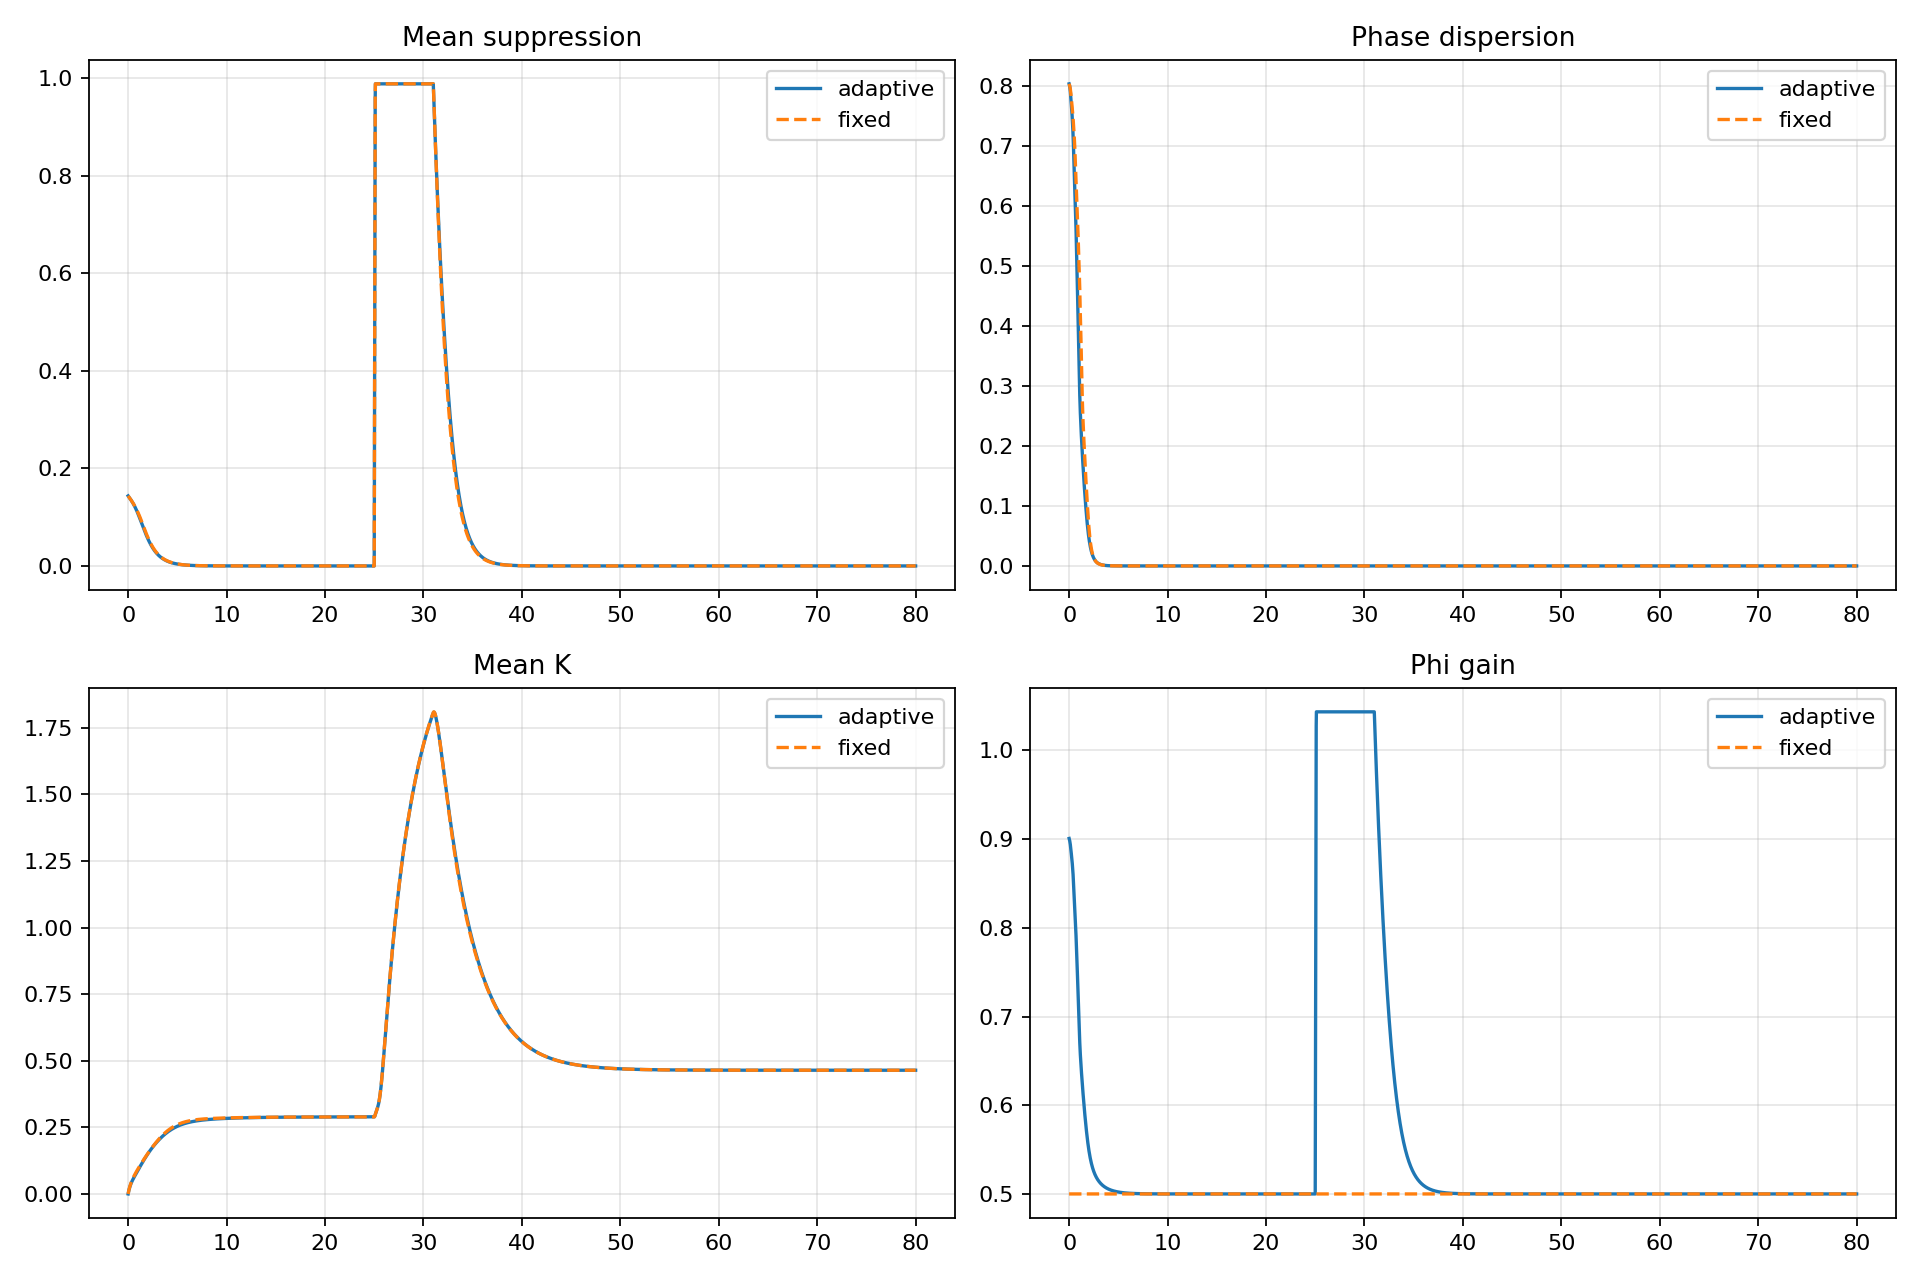
\includegraphics[width=0.95\linewidth]{figures/adaptive_rc_first_demo_plot.png}
    \caption{First adaptive RC sanity check versus fixed RC on a simple stress protocol.}
\end{figure}

The first tuning sweep on the symmetric toy group changed group recovery time but did not generate meaningful per-agent spread. After adding heterogeneous agent response, the trade-off became visible: a more spread-friendly controller increased the variance of individual recovery times while keeping the group recoverable. This supports the idea that adaptive success may be bounded resilience under diversity rather than minimizing a single mean time.
In the long-horizon multi-episode check, the group remained recoverable across all episodes, while group recovery time increased with episode index and the spread of individual recovery times stayed bounded. This is closer to a metastable picture: the controller does not erase diversity, but keeps the system in a live recoverable regime under repeated stress.
The spread-friendly preset showed a pronounced recovery tail, with early agents recovering much faster than the slowest ones, but without an uncontrolled cascade. This suggests contagion-like spreading of delay inside the crisis window, not a full group collapse.
The infection-over-time profile makes this explicit: after the stress ends, most agents remain above the suppression threshold for one to two time units, while a smaller tail persists longer. The spread-friendly preset keeps a larger delayed tail than the baseline, so it is more metastable in the sense of preserving diversity under stress, but not faster in mean recovery.
The long-term lag check shows that the control response is fast and bounded, but it does not yet improve across episodes. In other words, the controller is state-responsive rather than genuinely learning from past episodes. That is an important limit: the current adaptive RC sees the group and reacts, but does not yet accumulate memory of previous failures.
The first group-memory sweep suggests that $C_{\mathrm{crit}}\approx 0.60$ is a reasonable start: at that level, $K_g$ is activated only on the more informative episodes, rather than on every fluctuation. This is exactly the intended behavior for a group memory layer.
In the first integrated $K_g$ run, the gate opened only on the strongest later episodes, producing a small but real upward shift in $\phi_{\mathrm{gain}}$ and $\kappa$ without turning the controller into hard control. The effect is modest, which is expected for a first memory layer, but it confirms that the group memory can influence the coordinator only after meaningful episodes have accumulated.
When the $K_g$ influence was strengthened slightly, the adaptive gains increased further, but in the current toy setup the recovery tail and long-term lag did not change materially. This is a useful negative result: the memory layer affects control strength, but a stronger structural signal or longer horizon will likely be needed before it reshapes the recovery tail itself.
In the longer heterogeneous check, $K_g$ accumulated more strongly and shifted the average gains upward again, but the toy model still did not reorganize the tail geometry in a substantial way. This makes the next step clear: the memory layer is ready to be tested in the full networked setting, where spread, contagion, and lag should be more visible.
The first network-level test confirms the same qualitative picture: $K_g$ can accumulate strongly in a full network, but a single crisis window is still not enough to visibly change recovery time. This suggests that the memory layer is not broken; rather, it needs repeated stress episodes before it can alter the network tail in a measurable way.

\selectlanguage{russian}
\par
Первый tuning sweep на симметричной игрушечной группе изменил время восстановления группы, но не дал заметного разброса по отдельным агентам. После введения неоднородной реакции агентов trade-off стал видимым: более spread-friendly контроллер увеличил дисперсию индивидуальных времен восстановления, сохранив восстановимость группы. Это поддерживает идею, что успех adaptive-режима может заключаться в ограниченной живучести при разнообразии, а не в минимизации одного среднего времени.
В длинном проверочном прогоне с несколькими эпизодами группа оставалась восстановимой во всех эпизодах, тогда как время восстановления росло от эпизода к эпизоду, а разброс индивидуальных времен оставался ограниченным. Это уже ближе к метастабильной картине: контроллер не стирает разнообразие, но удерживает систему в живом, восстановимом режиме при повторном стрессе.
У spread-friendly preset виден выраженный хвост восстановления: ранние агенты выходят быстрее, а самые медленные существенно позже, но без неконтролируемой лавины. Это похоже на заражение задержкой внутри окна кризиса, а не на полный коллапс группы.
Профиль заражения во времени это показывает явно: после окончания стресса большинство агентов еще 1–2 единицы времени остаются выше порога подавления, а меньший хвост держится дольше. У spread-friendly хвост задержки больше, чем у baseline, так что он более метастабилен в смысле сохранения разнообразия под стрессом, но не быстрее по среднему восстановлению.
Проверка длинного лага показывает, что реакция контроллера быстрая и bounded, но не улучшается от эпизода к эпизоду. Значит, сейчас adaptive RC реагирует на состояние группы, но еще не накапливает память прошлых сбоев как отдельное обучение.
Первый свип по групповой памяти показывает, что $C_{\mathrm{crit}}\approx 0.60$ — разумный старт: при этом уровне $K_g$ активируется только на более информативных эпизодах, а не на каждой флуктуации. Это и есть нужное поведение для слоя групповой памяти.
В первой интеграции $K_g$ gate открылся только на сильных поздних эпизодах и дал небольшой, но реальный сдвиг вверх в $\phi_{\mathrm{gain}}$ и $\kappa$, не превращая контроллер в жесткий. Эффект пока умеренный, что нормально для первого слоя памяти, но он подтверждает, что групповая память может влиять на координатор только после накопления значимых эпизодов.
При небольшом усилении влияния $K_g$ adaptive gains выросли еще больше, но в текущей игрушечной постановке хвост восстановления и длинный лаг заметно не изменились. Это полезный отрицательный результат: слой памяти влияет на силу управления, но для изменения самого хвоста, вероятно, нужен более сильный структурный сигнал или более длинный горизонт.
В длинной неоднородной проверке $K_g$ накопился сильнее и снова поднял средние gains, но сама геометрия хвоста в игрушечной модели существенно не перестроилась. Это делает следующий шаг очевидным: слой памяти уже готов переноситься в полную сетевую постановку, где spread, contagion и lag должны проявиться намного лучше.
Первая сетевая проверка подтверждает ту же картину: $K_g$ может сильно накапливаться в полной сети, но одного кризисного окна еще недостаточно, чтобы заметно изменить время восстановления. Значит, память не сломана; ей просто нужен повторный стресс, чтобы повлиять на хвост сети измеримо.
\selectlanguage{english}


\section{Quantum QRC (Conceptual Bridge)}
We propose a quantum analogue of recognition and coherence-driven relaxation using a shared resonator as a soft metronome and sensor.

\paragraph{Resonator phase as metronome.}
Let $a$ be the cavity field. Define the global phase
\begin{equation}
\Phi = \arg\langle a\rangle.
\end{equation}
This provides a weak, global reference without projective measurement of individual phases.

\paragraph{Recognition without collapse.}
In dispersive coupling, a weak probe acquires a phase shift that depends on the qubit state. The effective match can be written as
\begin{equation}
\mathrm{match}_i \propto \mathrm{Re}\left(\langle \sigma_+^i\, a\rangle e^{-i\Phi}\right),
\end{equation}
which acts as a soft coherence indicator rather than a hard measurement.

\paragraph{Coherence-driven relaxation.}
Define dispersion via the resonator field,
\begin{equation}
\mathcal{D}=1-\left|\langle a\rangle\right|.
\end{equation}
Then a soft relaxation channel can be written as
\begin{equation}
\dot S_i \leftarrow \dot S_i - \gamma_{coh}(1-\mathcal{D})S_i.
\end{equation}
This yields recovery without strong forcing, analogous to the classical QRC mechanism.

\paragraph{Why this is new.}
The novelty is the combination: (i) soft metronome (resonator phase), (ii) recognition via weak phase shift, and (iii) coherence-driven relaxation, which together enable recovery from trapped states without hard resets.

\selectlanguage{russian}
\section{????????? QRC (?????????????? ????)}
?? ?????????? ????????? ?????? ????????????? ? ??????????? ?????????? ????? ????? ????????? ??? ?????? ???????? ? ??????.

\paragraph{???? ?????????? ??? ????????.}
????? $a$ ? ???? ??????????. ????????? ?????????? ????
\begin{equation}
\Phi = \arg\langle a\rangle.
\end{equation}
??? ???? ?????? ?????????? ?????? ??? ???????????? ????????? ??? ????????? ???????.

\paragraph{????????????? ??? ????????.}
? ???????????? ????? ?????? ???? ???????? ??????? ?????, ????????? ?? ????????? ??????. ??????????? match:
\begin{equation}
\mathrm{match}_i \propto \mathrm{Re}\left(\langle \sigma_+^i\, a\rangle e^{-i\Phi}\right),
\end{equation}
?????? ?????? ??????????? ??????????????? ?????? ???????? ?????????.

\paragraph{??????????? ??????????.}
????????? ????????? ????? ???? ??????????,
\begin{equation}
\mathcal{D}=1-\left|\langle a\rangle\right|.
\end{equation}
????? ?????? ????? ??????????:
\begin{equation}
\dot S_i \leftarrow \dot S_i - \gamma_{coh}(1-\mathcal{D})S_i.
\end{equation}
?? ???????????? ?????????????? ??? ???????? ????????????, ?????????? ????????????? QRC.

\paragraph{?????? ??? ????.}
??????? ? ?????????: (i) ?????? ???????? (???? ??????????), (ii) ????????????? ????? ?????? ??????? ?????, (iii) ??????????? ??????????. ?????? ??? ???? ????? ?? ???????????? ????????? ??? ??????? ???????.
\selectlanguage{english}

\section*{Open Additions}
Future work: explicit lag estimation, adaptive group-level delays, and hierarchical QRC (local + global).

\end{document}
